%%%%%%%%%%%%%%%%%%%%%%%%%%%%%%%%%%%%%%%%%
% Daily Laboratory Book
% LaTeX Template
%
% This template has been downloaded from:
% http://www.latextemplates.com
%
% Original author:
% Frank Kuster (http://www.ctan.org/tex-archive/macros/latex/contrib/labbook/)
%
% Important note:
% This template requires the labbook.cls file to be in the same directory as the
% .tex file. The labbook.cls file provides the necessary structure to create the
% lab book.
%
% The \lipsum[#] commands throughout this template generate dummy text
% to fill the template out. These commands should all be removed when 
% writing lab book content.
%
% HOW TO USE THIS TEMPLATE 
% Each day in the lab consists of three main things:
%
% 1. LABDAY: The first thing to put is the \labday{} command with a date in 
% curly brackets, this will make a new page and put the date in big letters 
% at the top.
%
% 2. EXPERIMENT: Next you need to specify what experiment(s) you are 
% working on with an \experiment{} command with the experiment shorthand 
% in the curly brackets. The experiment shorthand is defined in the 
% 'DEFINITION OF EXPERIMENTS' section below, this means you can 
% say \experiment{pcr} and the actual text written to the PDF will be what 
% you set the 'pcr' experiment to be. If the experiment is a one off, you can 
% just write it in the bracket without creating a shorthand. Note: if you don't 
% want to have an experiment, just leave this out and it won't be printed.
%
% 3. CONTENT: Following the experiment is the content, i.e. what progress 
% you made on the experiment that day.
%
%%%%%%%%%%%%%%%%%%%%%%%%%%%%%%%%%%%%%%%%%

%---------------------------------------------------------------------
%	PACKAGES AND OTHER DOCUMENT CONFIGURATIONS
%----------------------------------------------------------------------

\documentclass[idxtotoc,hyperref,openany,oneside]{labbook} % 'openany' here removes the gap page between days, erase it to restore this gap; 'oneside' can also be added to remove the shift that odd pages have to the right for easier reading

\usepackage[ 
  backref=page,
  pdfpagelabels=true,
  plainpages=false,
  colorlinks=true,
  bookmarks=true,
  pdfview=FitB]{hyperref} % Required for the hyperlinks within the PDF
  
\usepackage{booktabs} % Required for the top and bottom rules in the table
\usepackage{float} % Required for specifying the exact location of a figure or table
\usepackage{graphicx} % Required for including images
\usepackage{lipsum} % Used for inserting dummy 'Lorem ipsum' text into the template
\usepackage{mathrsfs}
\usepackage{amsmath}
\usepackage{soul}

\newcommand{\HRule}{\rule{\linewidth}{0.5mm}} % Command to make the lines in the title page
\setlength\parindent{0pt} % Removes all indentation from paragraphs

\usepackage{enumitem,amssymb}
\newlist{todolist}{itemize}{2}
\setlist[todolist]{label=$\square$}
\usepackage{pifont}
\newcommand{\cmark}{\ding{51}}%
\newcommand{\xmark}{\ding{55}}%
\newcommand{\done}{\rlap{$\square$}{\raisebox{2pt}{\large\hspace{1pt}\cmark}}%
  \hspace{-2.5pt}}
\newcommand{\wontfix}{\rlap{$\square$}{\large\hspace{1pt}\xmark}}
\newcommand{\tss}{\textsuperscript}
\newcommand{\tsbs}{\textsubscript}

%---------------------------------------------------------------------
%	DEFINITION OF EXPERIMENTS
%---------------------------------------------------------------------

\newexperiment{Notes}{Experiment Notes}
\newexperiment{Stock}{Stock creation}
\newexperiment{Process1Prep}{Preparation for Process 1}
\newexperiment{Process1_Fail}{Process 1 Mistake experiment}
\newexperiment{Process1_Fail_Counting}{Counting for Process 1
  Mistake experiment (Gamma)}
\newexperiment{Process1_Fail_Counting2}{Counting for Process 1
  Mistake experiment (Alpha)}
\newexperiment{Process1_Fail_Counting_Analysis}{Analysis
  for Process 1 Mistake (Gamma)}
\newexperiment{Cycle_X3_Prep}{Preparation for 3 Cycles}
\newexperiment{table1}{Isotopes we are looking for}
\newexperiment{Cycle_X3}{Cycle experiment, replicate of 3}
\newexperiment{programs}{Calculation Work}
%\newexperiment{shorthand}{Description of the experiment}

%----------------------------------------------------------------------
\begin{document}

%----------------------------------------------------------------------
%	TITLE PAGE
%-----------------------------------------------------------------------

\frontmatter % Use Roman numerals for page numbers
\title{
\begin{center}
\HRule \\[0.4cm]
{\Huge \bfseries Laboratory Journal }\\[0.4cm] % Degree
\HRule \\[1.5cm]
\end{center}
}
\author{\Huge Paul Mendoza \\ \\ \LARGE paul.m.mendoza@gmail.com \\[2cm]}
\date{This notebook begins 6 October 2016} 
\maketitle

\tableofcontents

\mainmatter 

%------------------------------------------------------------------------
%	LAB BOOK CONTENTS
%------------------------------------------------------------------------




%------------------------------------------------------------------------
%	LAB BOOK day
%-----------------------------------------------------------------------

\labday{Thursday, 6 October 2016\\ 8:30am - 11:00 am\\ 1:30pm - 3:30pm}

\experiment{table1}
\begin{itemize}
\item{Decay Monitors}
  \begin{itemize}
  \item{\tss{137}Cs/\tss{133}Cs}
  \end{itemize}
\item{Burnup Monitor}
  \begin{itemize}
  \item{(\tss{154}Eu/\tss{153}Eu) [\tss{155}Eu]}
  \end{itemize}
\item{Reactor type monitors}
  \begin{itemize}
  \item{(\tss{134}Cs/\tss{137}Cs)}
  \item{(\tss{150}Sm/\tss{149}Sm)}
  \item{(\tss{242}Pu/\tss{239}Pu)}
  \item{(\tss{135}Cs/\tss{137}Cs)}
  \item{(\tss{136}Ba/\tss{138}Ba)}
  \end{itemize}
\item{Isotope Solve list}
\end{itemize}

\begin{table}[H]
\begin{center}
\begin{tabular}{l l l}
\toprule
\tss{133}Cs & \tss{136}Ba & \tss{153}Eu\\ 
\tss{134}Cs & \tss{138}Ba & \tss{154}Eu\\
\tss{135}Cs & \tss{149}Sm & \tss{239}Pu\\
\tss{137}Cs & \tss{150}Sm & \tss{242}Pu\\
\bottomrule
\end{tabular}
\caption{Isotope solve list.}
\end{center}
\end{table}  

\experiment{Notes}

\begin{itemize}
\item{Project Number: 504370-0001}
\item{Files on computer saved in C:/Paul\_Mendoza}
\item{\tss{152}Eu Liquid calibration source}
  \begin{itemize}
  \item{Source 1577-22}
  \item{497.0 nCi}
  \item{Assy Date: 15 Feb 12}
  \item{1.00568g}
  \end{itemize}
\item{Stock HNO\tsbs{3}: Assuming Temp=24.8+/-3 $\rightarrow\boxed{Stock\ HNO_3}$}
  \begin{itemize}
  \item{Molarity : 15.35+/-0.13}
  \item{pH: -1.186+/-0.004}
  \item{Molality: 35.3+/-0.8}
  \item{Wt Concentration: 69.0+/-0.5}
  \item{Molar Mass: 63.0130+/-0.0012}
  \item{Density: 1.402+/-0.006}
  \end{itemize}
\item{Stock Iron Sulfamate $Fe(NH_2SO_3)_2$ $\rightarrow\boxed{Stock\ Fe(II)}$}
  \begin{itemize}
  \item{Molarity : 2.302+/-0.009}
  \item{Molality : 2.717+/-0.006}
  \item{Wt Concentration : 40.26+/-0.05}
  \item{Molar Mass : 248.022+/-0.017}
  \item{Density: 1.418+/-0.005}
  \end{itemize}
\end{itemize}

\experiment{Stock} % 

\begin{itemize}
\item{Get stock solution from Troy room 18A, store near rad waste}
\item{Grab 1000$\mu$l pipett from glovebox}
\item{Decontaminate with radic - dump waste into glass aq rad outside glove box}
\item{Practice pipetting 500$\mu$l to glass vial - setting 503 $\mu$l
  gives 500 $\mu$l}
\item{Class/lunch Break}
\item{Get alpha detector from Dr. Marianno}
\item{Set up laboratory notebook}
\item{Calculation}
  To do calculation to determine the volumes needed for a final
  concentration of a particular volume, knowing the initial
  concentrations
  \begin{align*}
    V_2&=\frac{b_2-\frac{M_1b_1}{A}}{M_2-\frac{M_1}{A}}\\
    V_1&=\frac{b-BV_2}{A}
  \end{align*}
  Where:
  \begin{align*}
    A&=(1-wt\%_1)\rho_1\\
    B&=(1-wt\%_2)\rho_2\\
    b_1&=(1-wt\%_3)V_3\rho_3\\
    b_2&=M_3V_3
  \end{align*}
  With known Molarity and volume of a solution
  how much, and of what concentration
  do we need to combine with a second solution
  to get a final solution of known concentration
  and volume?
  \begin{align*}
    B&=(1-wt\%_3)V_3\rho_3-(1-wt\%_1)V_1\rho_!\\
    A&=M_3V_3-M_1V_1\\
    C&=\frac{B}{A}=\frac{(1-wt\%_2)\rho_2}{M_2}
  \end{align*}
  Need iterative solution, choose:
  \begin{align*}
    M_2&=\frac{M_3V_3-M_1V_1}{V_3-V_1}\\
    V_2&=V_3-V_1
  \end{align*}
  Use to determine molality $\rightarrow$ $wt\%_2$ $\rightarrow$
  $\rho_2$. Then compare to $C$, iterate around the solution to
  find answer so that $C=\frac{(1-wt\%_2)\rho_2)}{M_2}$.
\end{itemize}

%------------------------------------------------------------------------
%	LAB BOOK day
%-----------------------------------------------------------------------

\labday{Friday, 7 October 2016\\ 9:00am - 12:00 am\\ 1:00pm - 4:00pm}

\experiment{Stock} % 

\begin{todolist}
\item[\done]{Program calculation for creation of stock - some
results shown below}
\item[\done]{Prepare shielding for transfer for closet solution}
  \begin{itemize}
  \item{Clean off and move leaded shielding in rad area to
    countertop next to fumehood}
  \item{Add diaper paper on countertop, and on shielding incase
    of contamination}
  \item{Practice transfer}
  \end{itemize}
\item[\done]{-}
\end{todolist}
\begin{center}
    0.149+/-0.011 ml of 15.43+/-0.06 M HNO\tsbs{3} $\boxed{Stock\ HNO_3}$\\
    +\\
    1.91+/-0.08  ml of 0.0+/-0 M solution $\boxed{DI\ Water}$\\
    = \\
    2.048+/-0.026 ml of 1.12+/-0.08 M HNO\tsbs{3}
  solution $\boxed{\rightarrow Stock}$ (glass container)
\end{center}
\begin{todolist}
\item[\done]{-}
\end{todolist}
\begin{center}
Combine 0.500+/-0.005 ml of 15.43+/-0.06 M HNO\tsbs{3}
solution $\boxed{closet}$\\
+\\
2.048+/-0.026 ml of 1.12+/-0.08 M HNO\tsbs{3} solution
$\boxed{Stock}$
\\
=\\
2.500+/-0.025 ml of 4.00+/-0.05 M HNO\tsbs{3} solution.
$\boxed{\rightarrow Stock}$
\end{center}

\begin{todolist}
\item[\done]{Lock $\boxed{Stock}$ in glovebox}
\item[\done]{Put Source back in rad closet}
\item[\done]{Clean up contamination added to pipette tip from transfer (for some reason, the contamination was added to the inside of the pipette itself, the tips used don't have the block, but still, none of the solution should have traveled up the shaft}
\item[\done]{Dispose of diaper paper laid down for transfer (where the glass bottle was set down which contained closet solution, there was contamination (the outside of the bottle of the closet solution is contaminated)}
\item[\done]{Move shielding back to where it was}
\end{todolist}

\experiment{Process1Prep}
\begin{todolist}
\item[\done]{Count calibration standard Eu-152 in HPGe 3 hours 22 minutes at furtherest position from detector (26 cm)}
  \begin{itemize}
  \item{Source 1577-22}
  \item{497.0 nCi}
  \item{Assy Date: 15 Feb 12}
  \item{1.00568g}
  \end{itemize}
\item[\done]{Create Eu-152 Excel Counting sheet template for standards}
\item[\done]{Set up ROI (region of interest) file for Eu-152}
\item[\done]{Start background count and done for the day}
  \begin{itemize}
  \item{Count lasted for 12 hours}
  \end{itemize}
\end{todolist}

%------------------------------------------------------------------------
%	LAB BOOK day
%-----------------------------------------------------------------------

\labday{Saturday, 8 October 2016\\ 10:00am - 2:00 pm}

\experiment{Process1Prep}

\begin{todolist}
\item[\done]{Finish background count, lasted 12 hours}
\item[\done]{Remove 0.3 ml from $\boxed{Stock}$ transfer to $\boxed{1}$
  for counting}
  \begin{itemize}
  \item{$\boxed{1}$ is a smaller tube, which will fit into a larger
    centrifuge tube for, well, centrifuging}
  \item{$\boxed{1}$ tube cannot fit into centrifuge tube with white
    push cap (pushes on outside of tube),
    white push cap is necessary when votex mixing, so a blue push cap
    (pushes on inside of tube), was put on for counting, these smaller
    tubes will have to have two caps following them around, I can't
    wait till the second cycle when the bigger tubes will be used}
  \item{Note for why smaller tubes are being used: when pipetting the
    smaller volume of 0.3 ml for aq/o phase separation it is much
    easier to have the smaller diameter tubes}
  \item{Stock was removed from glovebox, and after was put into the safe}
  \end{itemize}
\item[\done]{Count $\boxed{1}$ for 1 hour and 24 minutes}
\item[\done]{Fix density calculation in code, was slightly wrong before,
  this means $\boxed{Stock}$ and $\boxed{1}$ are slightly different
  from what they should be, but within error}
\item[\done]{Calculation for creation of Fe(II) solution (next page)}
\end{todolist}
\clearpage
\begin{center}
  $V_1$ ml of $M_{1,Fe}$ Fe(II) in $M_{1,HNO_3}$ HNO\tsbs{3}\\
  $+$\\
  $V_2$ ml of $M_{2,Fe}$ Fe(II) in $M_{2,HNO_3}$ HNO\tsbs{3}\\
  =\\
$V_3$ ml of $M_{3,Fe}$ Fe(II) in $M_{3,HNO_3}$ HNO\tsbs{3}.
\end{center}

The knowns are: \\
$M_{1,Fe}=2.302$, $\rho_1=1.418$, $M_{1,HNO_3}=0$ (Fe Stock soltuion)\\
$M_{2,Fe}=0$,$\rho_2=\rho_{HNO_3}(M_{2,HNO_3})$ \\
$V_3=4$ ml, $M_{3,Fe}=0.024$, $M_{3,HNO_3}=4$, $\rho_3=\rho_{HNO_3}(4M)$\\~\\

Mols of Fe(II) constant: $V_1=\frac{M_{3,Fe}V_3}{M_{1,Fe}}=0.042$\\
Mols of HNO\tsbs{3} constant: $V_2=\frac{V_3M_{3,HNO_3}}{M_{2,HNO_3}}$\\
Mass Constant: $V_2=\frac{V_3\rho_3-V_1\rho_1}{\rho_2}$\\~\\

Combine last two equations:$M_{2,HNO_3}-
\frac{V_3M_{3,HNO_3}\rho_2}{V_3\rho_3-V_1\rho_1}=0$\\~\\
Solve iteratively (where $M_{2,HNO_3}$ determines $\rho_2$)
with first guess of:
$M_{2,HNO_3}=\frac{M_{3,HNO_3}V_3}{V_2}$



%------------------------------------------------------------------------
%	LAB BOOK day
%-----------------------------------------------------------------------

\labday{Sunday, 9 October 2016\\ 7:30 pm - 11:30 pm}

\experiment{Process1Prep}

\begin{todolist}
\item[\done]{Prepare for multi contact extraction and back extraction exp}
  \begin{itemize}
  \item{Make solution of 30 vol.\% TBP with kerosene}
  \item{Make 40 ml of solution 4.06 M HNO\tsbs{3} solution, }
  \item{Transfer two smaller vials (one for TBP phase), one for
    Fe phase, with two different lids into glovebox (with
  a larger vial to hold them in the centrifuge)}
  \item{Transfer two smaller vials with centrifuge vials for
    centrifuging, keep one with water 0.3 ml, and TBP mix 0.32 ml
    $\boxed{Vial\ 1\ Budd}$, and
    the second with 1.2 ml of TBP mix and 1.25 ml water
    $\boxed{Vial\ 2\ Budd}$}
  \item{Transfer $\boxed{Stock}$ and $\boxed{1}$ to glovebox}
  \item{Transfer another vial to hold the Fe solution}
  \item{Make sure tweezers are in glovebox (they are) - to remove smaller
    vials from centrifuge tubes}
  \item{Transfer slightly contaminated pipette to glovebox}
  \item{All above vials that would contain solution were rinsed
    with whatever they would hold for approximately 3 minutes}
  \end{itemize}
\end{todolist}

\begin{todolist}
\item[\done]{-}
\end{todolist}
\begin{center}
15+/-0.15 ml of TBP $\boxed{Stock\ TBP}$\\
+\\
35+/-0.35 ml of kerosene $\boxed{Stock\ kerosene}$\\
=\\
50+/-0.5 ml of 30 vol.\% TBP.
$\boxed{\rightarrow TBP}$
\end{center}

\begin{todolist}
\item[\done]{-}
\end{todolist}
\begin{center}
10.579+/-0.011 ml of 15.35+/-0.13 M HNO\tsbs{3} $\boxed{Stock\ HNO_3}$\\
+\\
30.355+/-0.030 ml of 0.0+/-0 M HNO\tsbs{3} solution $\boxed{DI\ Water}$\\
=\\
39.94+/-0.14 ml of 4.07+/-0.04 M HNO\tsbs{3} solution
$\boxed{\rightarrow Fe\ Prep}$
\end{center}

To create an Fe solution for a back extraction, $\boxed{Fe\ Prep}$ should be
combined in the following manner (Small portions created because this
solution has a short half life with larger concentrations of $HNO_3$).

\begin{todolist}
\item{-}
\end{todolist}
\begin{center}
0.0417+/-0.0018 ml of 2.302+/-0.009 M Fe(II) in 0.0+/-0 M HNO\tsbs{3} $\boxed{Stock\ Fe(II)}$\\
+\\
3.941+/-0.027 ml of 0.0+/-0 M Fe(II) in 4.06+/-0.05 M HNO\tsbs{3} solution $\boxed{Fe\ Prep}$\\
+\\
4.000+/-0.020 ml of 0.0240+/-0.0010 M Fe(II) in 4.00+/-0.05 M HNO\tsbs{3} solution $\boxed{\rightarrow Bk\ Ex\ Solution}$.
\end{center}

\begin{todolist}
\item[\done]{Add Sodium Nitrite to $\boxed{1}$, it will sit overnight,
but it doesn't have to}
  \begin{itemize}
  \item{Dropped $\boxed{1}$, solution probably contaminated blue lid
    (crap), centrifuged on 1000 rpm for 2 minutes}
  \end{itemize}
\end{todolist}


%------------------------------------------------------------------------
%	LAB BOOK day
%-----------------------------------------------------------------------

\labday{Monday, 10 October 2016\\ 12:30 pm - 4:30 pm}

\experiment{Process1_Fail}
\begin{todolist}
\item[\done]{First contact - Extraction}
  \begin{itemize}
  \item{Add 0.32 ml $\boxed{TBP}$ to $\boxed{1}$}
  \item{Shake on Pulse Mode of 15 minutes on vortex mixer}
  \item{Change of plans (This occured while sample settled for
       a bit while changes were implemented)}
    \begin{itemize}
    \item{Put smaller tubes directly into centrifuge - so we do not
      have to switch caps so often}
    \item{Pulled out $\boxed{Vial\ 1\ Budd}$ and $\boxed{Vial\ 2\ Budd}$
      Pulled out of glovebox the smaller tubes,
      changed their caps, labeled them, put back into
      glovebox (5-10 minutes)}
    \end{itemize}
  \item{Centrifuge 1000 rpm for 10 minutes}
  \item{Attempted to pull out 0.30 ml of TBP phase}
    \begin{itemize}
    \item{Utter Failure}
    \item{Utter Failure again}
    \item{Utter failure...difficult to pull out 0.3 ml and keep
    phases separate}
    \end{itemize}
  \item{Added 1.08 ml $\boxed{TBP}$ to $\boxed{1}$ (for 0.2 ml buffer)}
    \begin{itemize}
    \item{All extractions at once (different from original exp)}
      \begin{align*}
        p=\frac{1}{1+\frac{1}{D}\frac{V_{aq}}{V_o}}
      \end{align*}
    \item{$V_o$ increased by fourfold}
    \item{Pipette slipped to 538 (instead of 540 $\rightarrow$ 0.4\%
      increase in error)}
    \end{itemize}
  \item{Vortex mix for 15 minutes on pulse mode}
  \item{Centrifuge 1000 cpm for 10 minutes}
  \item{Remove 1000 ml top phase (TBP), then remove
    another 200 ml of top phase (TBP) $\boxed{\rightarrow 2}$}
  \end{itemize}
\item[\done]{Creation of $\boxed{Bk\ Ex\ Solution}$}
\end{todolist}
\begin{center}
0.0417+/-0.0018 ml of 2.302+/-0.009 M Fe(II) in 0.0+/-0 M HNO\tsbs{3} $\boxed{Stock\ Fe(II)}$\\
+\\
3.941+/-0.027 ml of 0.0+/-0 M Fe(II) in 4.06+/-0.05 M HNO\tsbs{3} solution $\boxed{Fe\ Prep}$\\
+\\
4.000+/-0.020 ml of 0.0240+/-0.0010 M Fe(II) in 4.00+/-0.05 M HNO\tsbs{3} solution $\boxed{\rightarrow Bk\ Ex\ Solution}$.
\end{center}
\begin{todolist}
\item[\done]{Back Extraction - First Contact}
  \begin{itemize}
  \item{Add 1.4 $\boxed{Bk\ Ex\ Solution}$ to $\boxed{2}$}
  \item{Shake pulse mode for 15 minutes}
  \item{Remove 1.2 ml of bottom phase (Fe(II)) $\boxed{\rightarrow 3}$}
    \begin{itemize}
    \item{Lost two drops}
    \item{While placing vial into centrifuge, cap shot off,
      spraying solution everywhere...great}
    \end{itemize}
  \end{itemize}
\item[\done]{Back Extraction - Second Contact}
  \begin{itemize}
  \item{Add 1.2 $\boxed{Bk\ Ex\ Solution}$ to $\boxed{2}$}
  \item{Shake pulse mode for 15 minutes}
  \item{Remove 1.2 ml of bottom phase (Fe(II)) $\boxed{\rightarrow 3}$}
  \end{itemize}
\item[\done]{Back Extraction - Third Contact}
  \begin{itemize}
  \item{Add 1.2 $\boxed{Bk\ Ex\ Solution}$ to $\boxed{2}$}
  \item{Shake pulse mode for 15 minutes}
  \item{Remove 1.2 ml of bottom phase (Fe(II)) $\boxed{\rightarrow 3}$}
  \end{itemize}
\end{todolist}
\vspace{5mm}
This experiment had sputtering of pipette at certain times.

\experiment{Process1_Fail_Counting}
\begin{todolist}
\item[\done]{Counted waste $\boxed{1}$, containing 0.3
  ml of $\boxed{Stock}$ and 0.2 ml $\boxed{TBP}$, on HPGe,
  for 12 hours (left for the night)}
\end{todolist}

\begin{figure}[H] % Example of including images
\begin{center}
  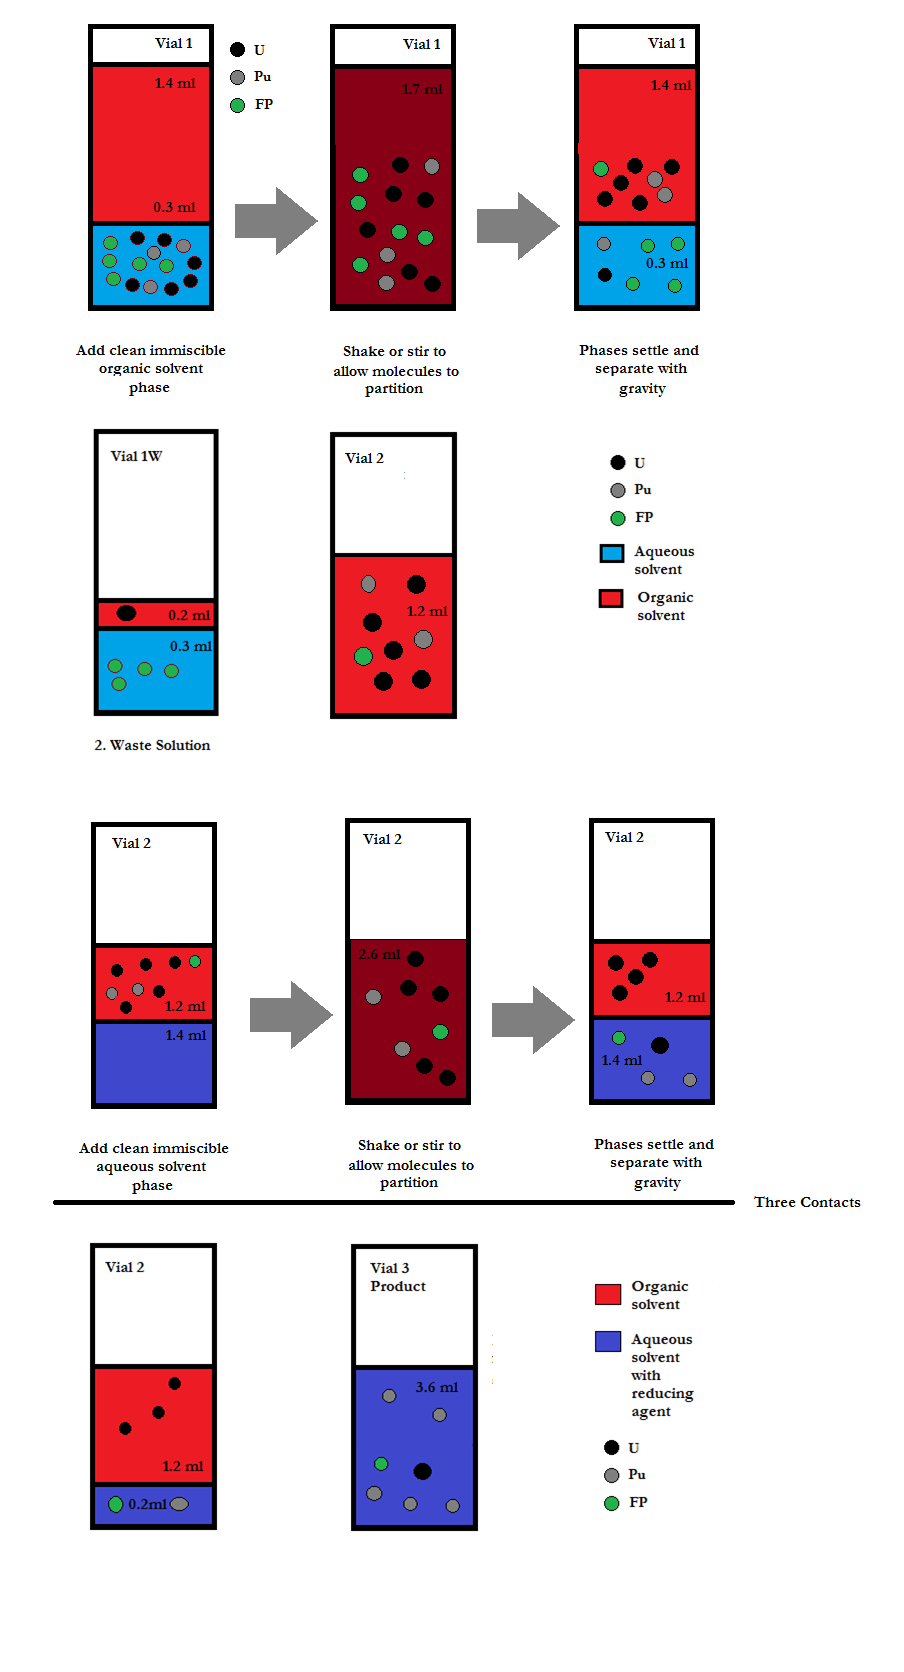
\includegraphics[width=0.85\linewidth]
                  {Figures/Process_1_Mess_Up}
\end{center}
\caption{Process 1 Mess Up Experimental Overview}
\label{fig:example2}
\end{figure}


%------------------------------------------------------------------------
%	LAB BOOK day
%-----------------------------------------------------------------------

\labday{Tuesday, 11 October 2016\\ 10:30 pm - 1:00 am}

\experiment{Process1_Fail_Counting}
There are 6 things to count.
\begin{todolist}
\item[\done]{Initial solution $\boxed{1}$ - 23 cm away, 0.3 ml HNO\tsbs{3}}
\item[\done]{Waste $\boxed{1}$ - 23 cm away, 0.3 ml HNO\tsbs{3} 0.2 ml TBP}
\item[\done]{Create 4 M HNO\tsbs{3} solution store in fume hood}
\end{todolist}
\begin{center}
2.6056+/-0.0026 ml of 15.35+/-0.13 M HNO\tsbs{3} solution $\boxed{Stock\ HNO_3}$\\
+\\
7.625+/-0.008 ml of 0.0+/-0 M HNO\tsbs{3} solution $\boxed{DI}$\\
+\\
9.985+/-0.035 ml of 4.01+/-0.04 M HNO\tsbs{3} solution $\boxed{\rightarrow 4\ M\ HNO_3}$.
\end{center}
\begin{todolist}
\item[\done]{Pull out 0.2 from bottom of $\boxed{1}$ (HNO\tsbs{3}),
  dillute to 0.3 ml with $\boxed{4\ M\ HNO_3}$ $\boxed{\rightarrow 1W}$ (Part)}
  \begin{itemize}
  \item{Count on HPGe $\sim$ 1 hour}
  \end{itemize}
\item[\done]{Pull out 0.3 ml from $\boxed{3}$ to count
  $\boxed{\rightarrow 3P}$ (product)}
  \begin{itemize}
  \item{Start Count on HPGe 4 hours (left overnight)}
  \end{itemize}
\item[\done]{Pull out 0.3 ml from top of $\boxed{2}$ (TBP), to count
       $\boxed{\rightarrow 2W}$ (Waste)}
\item{\st{Pull out 0.7 ml from top of $\boxed{2}$ (TBP)
  $\boxed{\rightarrow 2W2}$, then count $\boxed{2}$ - which should
    have 0.3 ml, 0.1 ml of TBP, and 0.2 ml of HNO}\tsbs{3}}
  \begin{itemize}
  \item{Coult not pull out all 0.7, but only 0.6}
  \end{itemize}
\item[\done]{Pull out 0.6 ml from top of $\boxed{2}$ (TBP)
  $\boxed{\rightarrow 2W2}$, should have 0.5 ml, 0.3 ml of TBP,
  and 0.2 ml of HNO\tsbs{3}}
\end{todolist}


\begin{figure}[H] % Example of including images
\begin{center}
  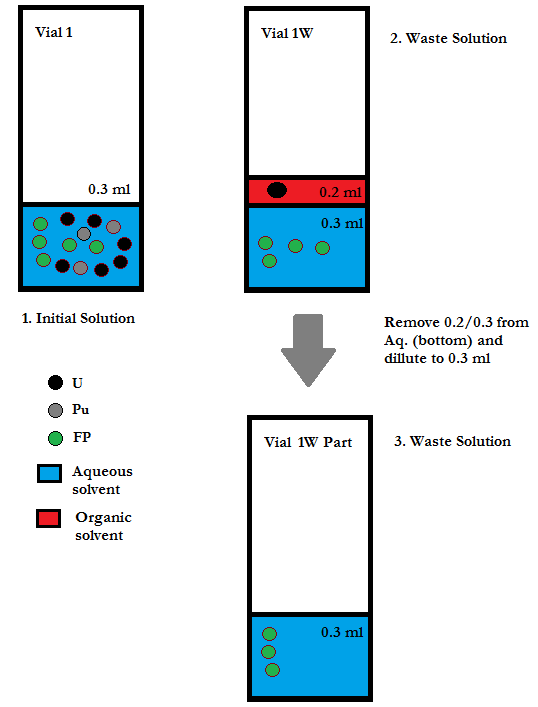
\includegraphics[width=0.5\linewidth]
                  {Figures/Extraction_Process_1_First_3_Counts}
\end{center}
\caption{First Three Counts}
\label{fig:example1}
\end{figure}

\begin{figure}[H] % Example of including images
\begin{center}
  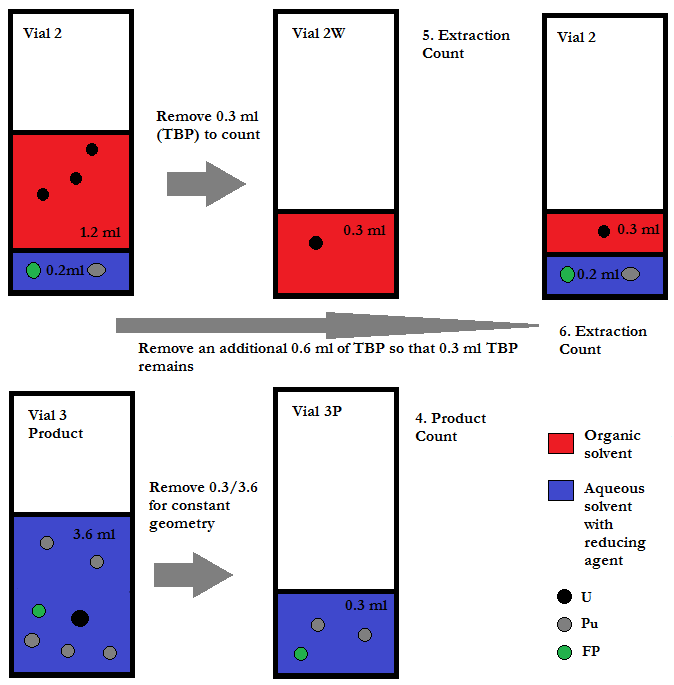
\includegraphics[width=0.5\linewidth]
                  {Figures/Back_Extraction_Process_1_Last_3_Counts}
\end{center}
\caption{Second Three Counts}
\label{fig:example2}
\end{figure}

%------------------------------------------------------------------------
%	LAB BOOK day
%-----------------------------------------------------------------------

\labday{Wednesday, 12 October 2016\\ 11:30 am - 1:30 pm}

\experiment{Process1_Fail_Counting}

\begin{todolist}
\item[\done]{Finish count $\boxed{3P}$}
\item[\done]{Start sample $\boxed{2W}$}
\item[\done]{Determine preliminary results}
  \begin{itemize}
  \item{Determined \tss{137}Cs, \tss{144}Ce, \tss{106}Rh
    activities for first 4 counts - Excel sheet}
  \item{Used excel sheet from John Burns for efficiency
    calibration of Eu-152 source...will just use
    the sheet from now on}
  \item{Also got from John, a templating file for GENIE,
    ``AnalysisMG.tpi'', which helps a lot for output from
    GENIE, again, something I do not want to modify}
  \item{The template was in an algorithm from GENIE, had
    the following steps}
    \begin{enumerate}
    \item{Peak Locate - Unidentified 2nd Diff}
      \begin{itemize}
      \item{Channels 1-16000}
      \item{2.50}
      \item{0.50 - FWHM}
      \item{Add to existing results}
      \end{itemize}
    \item{Peak Area - Sum/Non-linear LSQ Fit}
      \begin{itemize}
      \item{Channels 1-16000}
      \item{4 channels, use fixed tail parameters}
      \item{Channels, Step, 4.00, 4.00, 4.00}
      \item{Output to screen and printer}
      \end{itemize}
    \item{Reporting...}
      \begin{itemize}
      \item{``AnalysisMG.tpi'', ``C:/GENIE2K/CTLFILES/''}
      \item{PeakAnalysis, 1.000000}
      \item{Start on: Page One, New File, $\mu$Ci}
      \end{itemize}
    \end{enumerate}
  \end{itemize}
\item[\done]{Notes for research meeting}
  \begin{itemize}
  \item{Process dilutes by factor of 12, no matter what}
  \item{Concentrated stock by a factor of two}
  \item{Decreased initial volume}
  \item{Have to mainatin, 0.2 ml excess volume to pipette from top}
  \item{Have to maintain, 0.1 ml excess from bottom}
  \item{Mistake in extraction - all extractions at once}
  \end{itemize}
\end{todolist}



%------------------------------------------------------------------------
%	LAB BOOK day
%-----------------------------------------------------------------------

\labday{Thursday, 13 October 2016\\ 12:30 am - 4:30 pm}

\experiment{Process1_Fail_Counting}

\begin{todolist}
\item[\done]{Finish count $\boxed{2W}$}
\end{todolist}

\experiment{Process1_Fail_Counting2}
\begin{todolist}
\item[\done]{Start count $\boxed{2}$}
\item[\done]{Fix alpha counter, reivew alpha counting}
  \begin{itemize}
  \item{Alpha detector broken, fixed by plugging into proper port}
  \item{Counted Calibration Alpha source}
    \begin{itemize}
    \item{There are some details for determining
      what the alpha efficiency should be for the alpha
      detector, and I want to make sure I do it correctly,
      have not had time to look into it. I have a PDF file
      that shows what is in the sample\\
      /notebook/Figures/Alpha\_Copy.pdf}
    \item{Pu-239 and Pu-240 are unresolved}
    \item{Pu-238 and Am-241 are unresolved}
    \item{Isotope Droduets Laboratories}
    \item{38.81 nCi}
    \item{1451-68-3}
    \item{1 Dec 10}
    \item{Kevin also provided me with a Excel Sheet that does
      some of the calculations, probably will have to modify}
    \end{itemize}
  \end{itemize}
\item[\done]{Counted Alpha Background}
\item[\done]{Counted Alpha Calibration (9 mm position)}
\item[\done]{Prepare alpha sample of $\boxed{Stock}$}
  \begin{itemize}
    \item{From Jarrod's stock 10$\mu$l was dilluted to 1ml
    and 10 $\mu$l was taken}
  \end{itemize}
\end{todolist}
\begin{center}
10 $\mu$l of $\boxed{Stock}$ (4 M HNO\tsbs{3})\\
+\\
190 $\mu$l of DI water (leftover in glovebox)\\
=\\
0.2 ml of $\sim$ 0 M HNO\tsbs{3} $\boxed{4\ Dillution}$
\end{center}
\begin{todolist}
\item[\done]{Prepare and count alpha sample of Stock}
  \begin{itemize}
  \item{Take 20 $\mu$l of $\boxed{4\ Dillution}$, put onto
  concentric circle disk plates (innermost circle) $\boxed{D1}$}
    \begin{itemize}
    \item{It should be noted that once an alpha source is
      placed on these disks and dried out, they look no different
      from other disks}
    \end{itemize}
  \item{Let dry in glovebox}
  \end{itemize}
\item[\done]{Count $\boxed{D1}$ over night}
\end{todolist}

%------------------------------------------------------------------------
%	LAB BOOK day
%-----------------------------------------------------------------------

\labday{Friday, 14 October 2016\\ 8:30 am - 9:00 pm}

\experiment{Process1_Fail_Counting}

\begin{todolist}
\item[\done]{Finish count $\boxed{2}$}
\end{todolist}

\experiment{Process1_Fail_Counting2}
\begin{todolist}
\item[\done]{Finish count for $\boxed{D1}$}
\item[\done]{Move $\boxed{D1}$ to safe (or glovebox)}
\end{todolist}

\experiment{Process1_Fail_Counting_Analysis}
\begin{todolist}
\item{Attempt to understand our alpha efficiency (basically
  how much is in the calibration source)}
\end{todolist}

%------------------------------------------------------------------------
%	LAB BOOK day
%-----------------------------------------------------------------------

\labday{Monday - Wednesday, 17-19 October 2016}

\experiment{Process1_Fail_Counting_Analysis}

\begin{todolist}
\item{Looked into alpha calibration math some more}
\item[\done]{Analyze and automate (somewhat) Gamma analysis}
  \begin{itemize}
  \item{Program for pulling peak data from GENIE}
  \item{Program for calculating efficency from peak energy data using
    John Burn's Excel file}
  \item{Determine Compton Edges for peaks}
    \begin{itemize}
    \item{$$E_f=\frac{E_i}{1+\frac{E_i}{511}(1-cos\theta)}$$}
    \item{$$E_i=\frac{E_f}{1-\frac{E_f}{511}(1-cos\theta)}$$}
    \item{Found that I do not have any back scatter peaks}
    \end{itemize}
  \item{Program for finding sum peaks}
    \begin{itemize}
    \item{Included backscatter peaks}
    \item{Found some coincidence peaks, didn't know how to analyze}
    \end{itemize}
  \item{Quantify most of the peaks in gamma spectrum (took the longest)}
    \begin{itemize}
    \item{$$CPS=A\gamma\epsilon$$}
    \item{$$CPS=A_1\gamma_1\epsilon_1+A_2\gamma_2\epsilon_2$$}
    \item{Most peaks used the first equation, one peak had
      overlapping energies, so used the second equation,
      had to assume one of the activities}
    \end{itemize}
  \item{Applied this analysis to
    6 gamma spectrum (took second longest - now more automated)}
  \item{Create graphics to help depict
    what work was actually done}
  \end{itemize}
\item[\done]{Note: Follow these steps when analyzing Gamma}
  \begin{enumerate}
  \item{Make sure Efficiency Excel Sheet is up to date}
    \begin{itemize}
    \item{Run Eff Count and particular distance}
    \item{Run: ``Analyze - Execute Sequence - Analyze\_Data''
      on GENIE}
    \item{Save as a .PDF (not .pdf) file the spectra data
      : File - Export Report to PDF from GENIE}
    \item{Pull Peak information with Data\_Pull.py program (direct
    program to directory with .PDF file)}
    \item{Put data into spreed sheet
    ``C:/Rad\_Detection/Calibration/Gamma/Eff\_cal\_summary\_Eu-152.xlsm''}
    \end{itemize}
  \item{Gather data in a similar manner as with the efficiency count
  - will produce a bunch of plain Excel Sheets}
  \item{Find the template  from C:/Rad\_Dection folder, update
    real Eff column with ``Eff\_Calc.py'' (Make sure you
    copy paste energies into the gamma\_energies file)}
  \item{Copy this template over to the sheets you just made,
    and gamma analysis for the peaks will be complete}
    \begin{itemize}
    \item{Note: Will have to copy, paste, remove peak columns that
      were not found or in excess from template, lining up everything
      and then delete was copied over, then paste again, janky,
      but not super slow - this list is a reminder for Paul,
      if anyone else is using this list, would probably need
      more explanation }
    \end{itemize}
  \end{enumerate}
\item[\done]{Notes for Research Meeting}
  \begin{itemize}
  \item{Showed activities for each of the solutions}
  \item{Found that D-values couldn't be found because
    of experimental setup}
  \item{Activity Balance seemed to match up}
    \begin{itemize}
    \item{Although it wasn't perfect because the numbers
    weren't exactly close to zero, but within the error}
    \end{itemize}
  \item{Results seemed to match up with previous experiment}
  \item{Moving Forward, John and Sunil and I discussed
    what these next experiments should entail}
  \end{itemize}
\end{todolist}


%------------------------------------------------------------------------
%	LAB BOOK day
%-----------------------------------------------------------------------

\labday{Thursday, 20 October 2016}

\experiment{Cycle_X3_Prep}

Note from John:\\~\\
After the research meeting yesterday, I thought about Paul’s
project quite a bit and what the best path forward should be.
\textbf{In my opinion, it would be best for him to do a single-cycle}
\textbf{(extraction/back extraction) in a replicate of 3 and determine}
\textbf{the D-values for both the extraction and back extraction and}
\textbf{show the reproducibility of this single-cycle experiment.} I
believe this is one of the goal you set for him as a part of
his proposal. From there we can move into the whole process
with confidence that we have consistent behavior for Cs-137
and Cs-134, as well as, a good understanding of the D-values
for the isotopes of interest that can be seen by gamma-ray
analysis. He and I spent some time this morning talking about
this and we both agree that this week he will focus on completing
all 3 single-cycle replicates, gamma counting all the solutions,
alpha counting as many as possible (I do not believe alpha and
gamma counts cannot be performed at the same time, as they both
use the computer), and analyzing a majority of the data before
next week’s research meeting. If you do not think this is plan
of action in the best to pursue we can restructure it.
\\~\\
I spend the rest of the day doing homework, I aplogize,
but it was due yesterday, I think its dumb that I should
have to apologize for spending \textbf{ANY} time doing homework.
\\~\\
John also mentioned two good techniques, that should be noted:
\begin{itemize}
\item{Pipetting with equal volumes using the plastic squish tops}
  \begin{itemize}
  \item{Squeeze top while going through organic, suck up as much as
    possible}
  \item{Then draw from top as well}
  \end{itemize}
\item{Measureing volume with pipette}
  \begin{itemize}
  \item{The above technique would need some means for measuring volume
    using the pipette, you can vary the volume around
    what you thought you sucked up, and check if there is air
    at the bottom of the tip}
  \end{itemize}
\end{itemize}


%------------------------------------------------------------------------
%	LAB BOOK day
%-----------------------------------------------------------------------

\labday{Friday, 21 October 2016\\ 9:30am - 12:00 pm\\1:00 pm 6:00 pm}

\begin{todolist}
\item[\done]{Updated this lab notebook (most of this morning)}
\end{todolist}

\experiment{Cycle_X3_Prep}

\begin{todolist}
\item[\done]{Practice pipetting out with squish tops like John Mentioned}
  \begin{itemize}
  \item{Used Kerosene solution, used squish pipettes and variable
    pipettes - settled upon using 500 $\mu$l
    and taking out 350 $\mu$l and then
    getting as much out as possible with the squish pipette -
    I get about 450 $\mu$l of bottom phase (HNO\tsbs{3})
    and 425 $\mu$l of top phase (TBP)}
  \item{Determine if 0.3 ml is a good amount of solution to use}
  \item{Switching to 0.5 ml, keeping smaller vials}
  \end{itemize}
\item[\done]{Create and label vials $\boxed{5}$ $\boxed{6}$ and
  $\boxed{7}$ to hold stock solution. Did not leech them,
  hopefully barium contamination wont be a huge deal,
  we will assume all the data for Cs can be gathered from \tss{133}Cs.}
\item[\done]{Transfer 0.5 ml of $\boxed{Stock}$ to $\boxed{5}$}
\item[\done]{Transfer 0.5 ml of $\boxed{Stock}$ to $\boxed{6}$}
\item[\done]{Transfer 0.5 ml of $\boxed{Stock}$ to $\boxed{7}$}
\item[\done]{Add scoop of sodium nitrite to $\boxed{5}$}
\item[\done]{Add scoop of sodium nitrite to $\boxed{6}$}
\item[\done]{Add scoop of sodium nitrite to $\boxed{7}$}
\item[\done]{Centrifuged $\boxed{5}$, $\boxed{6}$
  and $\boxed{7}$ to push all solution to
  botttom of vials}
\item[\done]{Start count of $\boxed{5}$ noticed bubbles in solution,
  might have to recount - left overnight}
\end{todolist}

\experiment{Process1_Fail_Counting2}

\begin{todolist}
\item[\done]{Took 20 $\mu$l out of $\boxed{3}$ and put
  onto planchet chip (no dillution)}
  \begin{itemize}
  \item{Moved chip too early (before drying, ruined
    detector volume)}
  \item{Made another source with an additional 20 $\mu$l,
    letting it dry over night}
  \end{itemize}
\end{todolist}



%------------------------------------------------------------------------
%	LAB BOOK day
%-----------------------------------------------------------------------

\labday{Saturday, 22 October 2016\\ 3:30 pm - 3:45 pm\\ 8:00 pm - 8:30 pm}

\experiment{Cycle_X3_Prep}

\begin{todolist}
\item[\done]{Finished count for $\boxed{5}$}
\item[\done]{Started count of $\boxed{6}$}
  \begin{itemize}
  \item{Switching from push clear caps to blue push caps}
  \item{This sample had less bubbles than the one yesterday}
  \end{itemize}
\item[\done]{Finished count of $\boxed{6}$}
  \begin{itemize}
  \item{Some liquid was not at the bottom of the vial,
    messing with geometry, centrifuged with $\boxed{7}$
    might have to recount}
  \end{itemize}
\item[\done]{Started count of $\boxed{7}$}
  
\end{todolist}

%------------------------------------------------------------------------
%	LAB BOOK day
%-----------------------------------------------------------------------

\labday{Sunday, 23 October 2016}

\experiment{Cycle_X3_Prep}

\begin{todolist}
\item[\done]{Finished count $\boxed{7}$}
\item[\done]{Analyzed Counts from $\boxed{5}$, $\boxed{6}$, and
  $\boxed{7}$}
  \begin{itemize}
  \item{Did not like how $\boxed{6}$ didn't fit with others}
  \end{itemize}
\item[\done]{Started recount of $\boxed{6}$}
\item[\done]{Start Excel Sheet for analysis and
           write program for quicker gamma analysis}
\end{todolist}

%------------------------------------------------------------------------
%	LAB BOOK day
%-----------------------------------------------------------------------

\labday{Monday, 24 October 2016\\10:00 am - 12:00 pm\\3:00 pm -
        8:00 pm}

\experiment{Cycle_X3_Prep}

\begin{todolist}
\item[\done]{Finished count $\boxed{6}$}
\item[\done]{Transfer:}
  \begin{itemize}
  \item{Vials labeled $\boxed{5\ Aq}$, 
    $\boxed{5\ Or}$, $\boxed{6\ Aq}$, $\boxed{6\ Or}$,
    $\boxed{7\ Aq}$, $\boxed{7\ Or}$}
  \item{With clear push lids, and blue push lids (named)}
  \item{Squish pipettes}
  \end{itemize}
  Into glovebox small antichamber
\item[\done]{$\boxed{5}$, $\boxed{6}$, and $\boxed{7}$ already
  in antichamber}
\item[\done]{Transfer vials with clear lids into glovebox, but
  leave the blue lids in the antichamber (lid transfer area)}
\item[\done]{Dump $\boxed{Back\ Ex\ Solution}$ into aqeuous
  waste ($\sim$ 0.2 $\mu$l) (decays - will prepare a fresh batch)}
\end{todolist}

\experiment{Process1_Fail_Counting2}

\begin{todolist}
\item[\done]{Moved alpha sample to count on PIPS detector}
  \begin{itemize}
  \item{Saw energy smearing for counts}
  \item{Preliminary results are what was expected if
    we take a larger range of counts}
  \end{itemize}
\end{todolist}

\experiment{Cycle_X3}

\begin{todolist}
\item[\done]{Add 500$\mu$l TBP to $\boxed{5}$, $\boxed{6}$,
  $\boxed{7}$}
\item[\done]{Shake $\boxed{5}$ on Pulse mode for 15 minutes}
\item[\done]{Shake $\boxed{6}$ on Pulse mode for 15 minutes}
\item[\done]{Shake $\boxed{7}$ on Pulse mode for 15 minutes}
\item[\done]{Create $\boxed{EX Buddy}$ so all samples can be
  centrifuged together}
  \begin{itemize}
  \item{500 $\mu$l of 4 M HNO\tsbs{3} + 500 $\mu$l of 30 vol.\%
    TBP}
  \end{itemize}
\item[\done]{Centrifuge samples for 30,000 rpm for 5 minutes}
\item[\done]{Separate phases for samples}
  \begin{itemize}
  \item{A total of 4 drops were dropped in this process}
    \begin{enumerate}
    \item{Sample $\boxed{5}$ aqueous transfer}
    \item{Sample $\boxed{6}$ organic transfer}
    \item{Sample $\boxed{7}$ aqueous and organic transfer}
    \end{enumerate}
  \item{Using a variable pipette and the squish pipette,
    as much of the top phase (organic) phase was removed as possible
    (turns out to be around 450 $\mu$l and transfered to
    $\boxed{5\ Or}$, $\boxed{6\ Or}$, and $\boxed{7\ Or}$.}
  \item{Then as much of the bottom phase (aqueous) was removed as
    possible (turns out to be around 430 $\mu$l) and transfered
    to $\boxed{5\ Aq}$, $\boxed{6\ Aq}$, and $\boxed{7\ Aq}$.}
  \end{itemize}
\item[\done]{Measure Volumes of 9 vials (Aqueous, organic, and original
  - units of $\mu$l)}
  \begin{itemize}
  \item{Clean outside of vials before taking volume measurements}
  \item{Centrifuge vials before taking volume measurements}
  \item{Google says that 1 drop of water is about 50 $\mu$l}
  \end{itemize}
\end{todolist}
\begin{center}
  \begin{tabular}{||c c c c c c||}
    \hline
    Series & Aqueous & Organic & Original & Should Add To & Missing\\ [0.5ex]
    \hline\hline
    5 & 461+/-9.22 & 430+/-8.6 & 55+/-5 & 1000+/-7.1 & 54+/-15.3\\
    \hline
    6 & 469+/-9.38 & 430+/-8.6 & 53+/-5 & 1000+/-7.1 & 48+/-15.4\\
    \hline
    7 & 469+/-9.38 & 430+/-8.6 & 57.5+/-5 & 1000+/-7.1 & 43.5+/-15.4\\
    \hline
  \end{tabular}
\end{center}

\begin{todolist}
\item[\done]{Count $\boxed{7\ Or}$ 12:00 pm - 6:00 pm}
\item[\done]{Start count $\boxed{7\ Or}$ on face of detector 6:00 pm
  this is because I cannot see \tss{134}Cs - the isotope I am
  most concerned about}
  \begin{itemize}
  \item{Will try and implement this:}
    $$CPS=A\epsilon_D\epsilon_G\gamma$$
    Where:
    \begin{center}
    $\epsilon_D=$Detector eff\\
    $\epsilon_G=$Geometric eff\\
    $\gamma=$yield\\
      $A=$activity
    \end{center}
    At two different distances $1$ and $2$:
    \begin{align*}
      CPS_1&=A\epsilon_D\epsilon_{G1}\gamma\\
      CPS_2&=A\epsilon_D\epsilon_{G2}\gamma
    \end{align*}
    Take ratio:
    \begin{equation*}
      \frac{CPS_1}{CPS_2}=\frac{A\epsilon_D\epsilon_{G1}\gamma}
           {A\epsilon_D\epsilon_{G2}\gamma}=
           \frac{\epsilon_D\epsilon_{G1}}{\epsilon_D\epsilon_{G2}}
           =R
    \end{equation*}
    Kept both efficiencies because calibration lumps both together.
    If This ratio, $R$ is known, then we can count at a closer
    distance and say:
    \begin{equation*}
      CPS_2=\frac{CPS_1}{R}
    \end{equation*}
  \end{itemize}
\item[\done]{Move $\boxed{6\ Or}$ and $\boxed{7\ Aq}$ to Antichamber
  (not sure which one I am counting next)}
\end{todolist}

\experiment{programs}
\begin{todolist}
\item[\done]{Modify program for analyzing spectra}
  \begin{itemize}
  \item{Hopefully now analyzing gamma data will just be,
    run program, and copy a part of an excel spreedsheet}
  \end{itemize}
\end{todolist}

%------------------------------------------------------------------------
%	LAB BOOK day
%-----------------------------------------------------------------------

\labday{Tuesday, 25 October 2016\\8:00 am}


\experiment{Cycle_X3}


\begin{todolist}
\item[\done]{Count $\boxed{6\ Or}$ 8:00 pm - 11:00 am}
\item{\st{Go to count $\boxed{5\ Or}$}}
  \begin{itemize}
  \item{Have $\boxed{7\ Or}$ and $\boxed{7\ Aq}$ in small
    antichamber}
  \item{Put antichamber to vacuum to transfer vials into
    glovebox}
  \item{Push caps exploded off vials due to large pressure
    difference...that is very dissapointing}
  \end{itemize}
\item[\done]{Clean up contamination from exploded vials in antichamber}
  \begin{itemize}
  \item{Dispose of counting vials, and caps for all vials rad waste}
  \item{Dispose of exploded vials in rad waste (after dried)}
  \item{Remove diaper paper from transfer plate}
  \item{Clean with radiac wipes}
    \begin{itemize}
    \item{Clean antichamber}
    \item{Clean antichamber}
    \item{Swipe area, count on alpha detector, because
      our swipe counter is down}
    \item{Clean antichamber}
    \item{Dr. Chirayath brought someone by to talk, not a good time}
    \item{Clean antichamber}
    \item{Clean glass beaker that was in antichamber...lots}
    \end{itemize}
  \item{Final areas swiped and counted for 10
    minutes after decontamination}
    \begin{itemize}
    \item{Tray $\sim$0 counts in alpha realm}
    \item{Top part of cylinder of antichamber
      $\sim$3 counts in alpha realm (around 20 for background)}
    \item{Top back part of cylinder $\sim$ 100 - still slightly
      contaminated, but no time for continued cleaning,
      because need to do experiment}
    \item{Left/Right side of cylinder (mid plane) $\sim$ small}
    \item{Bottom back portion of cylinder of antichamber - $\sim$100}
    \item{Glass vial - none}
    \end{itemize}
  \end{itemize}
\item[\done]{Count $\boxed{5\ Or}$ 3:00 pm - 7:30 pm (finally!!)}
\item{\st{Count $\boxed{7\ Aq}$ 9:00 pm - 11:00 pm} (Spilled)}
\item[\done]{Count $\boxed{6\ Aq}$ 7:00 pm - 9:00 pm}
\item[\done]{Count $\boxed{5\ Aq}$ 9:00 pm - 8:00 am}
\end{todolist}
\begin{todolist}
\item[\done]{-}
\end{todolist}
\begin{center}
0.0417+/-0.0018 ml of 2.302+/-0.009 M Fe(II) in 0.0+/-0 M HNO\tsbs{3} $\boxed{Stock\ Fe(II)}$\\
+\\
3.941+/-0.027 ml of 0.0+/-0 M Fe(II) in 4.06+/-0.05 M HNO\tsbs{3} solution $\boxed{Fe\ Prep}$\\
+\\
4.000+/-0.020 ml of 0.0240+/-0.0010 M Fe(II) in 4.00+/-0.05 M HNO\tsbs{3} solution $\boxed{\rightarrow Bk\ Ex\ Solution}$.
\end{center}
\begin{todolist}
\item[\done]{Add 430 $\mu$l Fe(II) solution to $\boxed{5\ Or}$}
\item[\done]{Add 430 $\mu$l Fe(II) solution to $\boxed{6\ Or}$}
\item{\st{Add XX $\mu$l Fe(II) solution to $\boxed{7\ Or}$} (spilled)}
\item[\done]{Shake $\boxed{5\ Or}$ 15 minutes on pulse mode}
\item[\done]{Shake $\boxed{6\ Or}$ 15 minutes on pulse mode}
\item{\st{Shake $\boxed{7\ Or}$ 15 minutes on pulse mode} (spilled)}
\item{\st{Remove XX $\mu$l organic and XX $\mu$l aqueous
  from $\boxed{Ex\ Buddy}$} (No longer necessary)}
\item[\done]{Centrifuge $\boxed{5\ Or}$, $\boxed{6\ Or}$, \st{$\boxed{7\ Or}$}
  \st{$\boxed{Ex\ Buddy}$}, 30,000 rpm for 5 minutes}
\end{todolist}
\begin{todolist}
\item[\done]{Vials labeled $\boxed{5\ AqII}$, 
  $\boxed{5\ OrII}$, $\boxed{6\ AqII}$, $\boxed{6\ OrII}$,
  \st{$\boxed{7\ AqII}$, $\boxed{7\ OrII}$}, transfered into
  glovebox}
\item[\done]{Separate phases for samples}
  \begin{itemize}
  \item{A total of 1 drops were dropped in this process}
    \begin{enumerate}
    \item{Sample $\boxed{5\ Or}$ aqueous or organic transfer}
    \end{enumerate}
  \item{Using a variable pipette and the squish pipette,
    as much of the bottom phase (aqueous) phase was removed as possible
    and transfered to
    $\boxed{5\ OrII}$, $\boxed{6\ OrII}$, and \st{$\boxed{7\ OrII}$}.}
  \item{Then as much of the top phase (organic) was removed as
    possible and transfered
    to $\boxed{5\ AqII}$, $\boxed{6\ AqII}$, and \st{$\boxed{7\ AqII}$}.}
  \end{itemize}
\item[\done]{Measure Volumes of 9 vials (Aqueous, organic, and original
  - units in $\mu$l)}
\end{todolist}
\begin{center}
  \begin{tabular}{||c c c c c c||}
    \hline
    Series & Aqueous II & Organic II & Original II & Should Add to
    & Missing\\ [0.5ex]
    \hline\hline
    5 & 407+/-8.14 & 380+/-7.6 & 38+/-5 & 860+/-12.2 & 35.0+/-17.2\\
    \hline
    6 & \st{402}415+/-8.3 & \st{360}380+/-7.6 & 35+/-5 & 860+/-12.2
    & 30+/-17.3\\
    \hline
  \end{tabular}
\end{center}

\experiment{programs}

\begin{todolist}
\item[\done]{Updated Spreedsheets to calculate
  activities based on avaiable peaks, also if
  a particular peak has really large errors,
  this will be ignored. Also updated Excel sheets
  to calculate propagated error mass in each vial
  - for D-value calculations}
  \begin{equation*}
    grams=\frac{\text{Activity}\times\text{Molar Mass}}
    {\lambda_sN_A}
  \end{equation*}
  where $\lambda$ is in seconds and $N_A$ is avogadros number.
\end{todolist}



%------------------------------------------------------------------------
%	LAB BOOK day
%-----------------------------------------------------------------------

\labday{Wednesday, 26 October 2016\\8:00 am}


\experiment{Cycle_X3}

\begin{todolist}
\item{Finish count $\boxed{5\ Aq}$}
\item{Count Vials}
\item{Analyze spectra}
\end{todolist}



%----------------------------------------------------------------------
%	Examples
%-----------------------------------------------------------------------
%---------------------------------------
% Blank template to use for new days:
%---------------------------------------
%\labday{Day, Date Month Year}
%\experiment{}
%Text

%---------------------------------------
% To do list
%---------------------------------------
%% \begin{todolist}
%% \item[\wontfix]{profit}
%% \item[\done]{This is done}
%% \item{This is not done}
%% \end{todolist}

%---------------------------------------
% Vial Step
%---------------------------------------
%% \begin{todolist}
%% \item{-}
%% \end{todolist}
%% \begin{center}
%% Vial 1\\
%% +\\
%% Vial 2\\
%% =\\
%% Final Vial
%% \end{center}

%% \labday{Example} % We don't want a date here so we make the labday blank

%% \begin{center}
%% \HRule \\[0.4cm]
%% {\huge \textbf{Examples}}\\[0.4cm] % Heading
%% \HRule \\[1.5cm]
%% \end{center}

%% %-----------------------------------------------------------------------
%% %	Formulae
%% %-----------------------------------------------------------------------
%% \huge \textbf{Formulae} \\ \\

%% \normalsize \textbf{Formula 1 - Pythagorean theorem}\\ \\
%% $a^2 + b^2 = c^2$\\ \\

%% %--------------------------------------------------------------
%% %	Citation
%% %--------------------------------------------------------------

%% Citation test \cite{Tatro2013}.

%% %--------------------------------------------------------------
%% %	Figure
%% %--------------------------------------------------------------

%% \begin{figure}[H] % Example of including images
%% \begin{center}
%% 
\includegraphics[width=0.5\linewidth]{Figures/example_figure}
%% \end{center}
%% \caption{Example figure.}
%% \label{fig:example_figure}
%% \end{figure}

%% %--------------------------------------------------------------
%% %	Table
%% %--------------------------------------------------------------

%% \experiment{table}

%% \begin{table}[H]
%% \begin{tabular}{l l l}
%% \toprule
%% \textbf{Groups} & \textbf{Treatment X} & \textbf{Treatment Y} \\
%% \toprule
%% 1 & 0.2 & 0.8\\
%% 2 & 0.17 & 0.7\\
%% 3 & 0.24 & 0.75\\
%% 4 & 0.68 & 0.3\\
%% \bottomrule
%% \end{tabular}
%% \caption{The effects of treatments X and Y on the four groups studied.}
%% \label{tab:treatments_xy}
%% \end{table}

%% Table \ref{tab:treatments_xy} shows that groups 1-3 reacted similarly to the two treatments but group 4 showed a reversed reaction.

%% %------------------------------------------------------------
%% %	Bibliography
%% %------------------------------------------------------------
%% \bibliography{references} 
%% \bibliographystyle{plain} 

\end{document}

